\section{Kinect Software}\label{Software}

%(Essenz auf dem, was Kinect für mich erledigt theorie, mathematische Berechnung tiefe und skeletonstream usw)

%Rauminformationen für Software
%Vorteil: Günstig, leicht zu entwickeln, da SDK vorhanden

%Da das Produkt Xbox Kinect bereits vor einigen Jahren auf den Markt kam, hatten die Entwickler Zeit, um ein SDK zu entwickeln, was alle wichtigen Programmfunktionen bereits enthält. Dies macht es einem Entwickler relativ leicht eine Anwendung zu erstellen, die bestimmte Kinect-Funktionen bereitstellt. 

%	
%	Depth Stream
%		RAW Data Array (KINECT FOR WINDOWS SDK PROG GUIDE)
%		Im Grunde Grundlage für Skeleton Stream
%		Depth-Range (u.a. auch Near Mode)
%		Mehrere Spieler (Playerindex)
%
%
%	Skeleton Stream
%		+ Bild 
%		Benutzt Tiefenstream
%		Kinect Raum (Koord.)
%		+ Bild
%		Algorithmus mit Farben
%		Color Regions (PDF HOW DOES KINECT WORK)
%		Joints
%		Bone Sequence
%		Skeleton Smoothing, Jitter
%
%
%	Fazit: Habe Skelett. Extrahiere Winkel, Gebe Nao

Die im vorigen Kapitel aufgezeigte Hardware liefert die entsprechenden Sensorinformationen, die nun
softwaretechnisch zu einer abstrakteren Ebene zusammengefasst werden müssen. Die Funktion dieser
Verarbeitungen speziell für das Microsoft Kinect SDK soll in diesem Kapitel erläutert werden.

\begin{description}
	\item[Die Hardware liefert folgende Werte:]~\par
	\begin{itemize}
		\item RGB Bildsignal der Kamera
		\item Tiefenwerte
		\item Audiosignale inkl. Richtungswert des Microphonarrays
	\end{itemize}
\end{description}

\noindent
Wie bereits erwähnt sind die Audiodaten für dieses Projekt jedoch irrelevant. Wichtig sind primär die Bilddaten inklusive Tiefenwerte.
Das Kinect SDK bietet bereits standardmäßig Zugriff auf diese Werte. Dabei können im Programm bestimmte Proxyobjekte registriert und abgefragt werden. Wie diese im Programm letztendlich verwendet werden,
wird im folgenden Kapitel \ref{SDK} \nameref{SDK} näher erläutert. Dieses Kapitel beschäftigt sich
damit, wie diese Funktionen im Inneren funktionieren.

\subsection{Der Tiefenstream}
Der Tiefenstream (Depth-Stream) liefert zu jedem Pixel einen Tiefenwert. Dieser Wert representiert
die Entfernung zu dem jeweiligen Objekt. Damit ist das am nächsten befindliche Objekt gemeint,
da verdeckte Objekte nicht vom Sensor erkannt werden.
Aus diesem Stream kann man beispielsweise ein Tiefenbild mit verschiedenen Grauwerten generieren, die representativ für die Entfernung zur Kinect stehen. Die Depth-Stream Daten werden in einem 16 Bit Array transportiert. Dabei sind 3 untersten Bits jedoch für die Erkennung von mehreren Spielern reserviert
(Siehe Kapitel \ref{skeleton} \nameref{skeleton}). Die oberen 13 Bit enthalten die eigentlichen Tiefendaten. Ein solcher Tiefenstream kann wie folgt aussehen:

%Einfuegen: Bild mit Tiefenstream

Für dieses Projekt ist das Skeletonobjekt von großer Bedeutung. Anhand von Vergleichsmustern erzeugt die Software -nicht Kinect!- einen sog. Skeletonstream, der versucht die Position eines menschlichen Skeletts im Kinect Koordinatenraum abzubilden.\cite{SWB-376536934}

\subsection{Der Skeletonstream}\label{skeleton}
Damit die Bewegungen eines Benutzers mittels Kinect erkannt und im Programm verarbeitet werden können, werden im Tiefenstream bestimmte Bereiche definiert und mit bestehenden Mustern verglichen. Somit können die einzelnen Gelenke des menschlichen Skeletts (Joints) erkannt und in Zusammenhang gebracht werden. Als Entwickler können diese dann in einem Skelettobjekt mit der erkannten Genauigkeit ausgelesen und verwendet werden. Für die Erkennung der Armbewegungen werden Schulter-, Ellenbogen-, Hand- und Hüftjoints benötigt (Siehe Realisierung).

\begin{figure}[H]						
	\centering							
	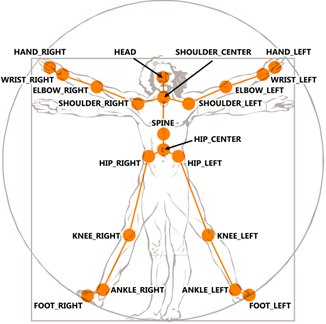
\includegraphics[scale=1.0]{Bilder/kinect_joints.png}			
	\caption{Kinect Joints \cite{ws:microsoft_jointType}}						
	\label{f:kinect_joints}						
\end{figure}



(Technischer Hintergrund der Berechnung -> Bild mit verschiedenen Farben für SKelettbereiche, aber nicht öffentlich, da Microsoft Geheimnis)

(Bild Kinect Koordinatenraum)
(Bild mehrere User im Kinectraum)

\todo{SDK Funktionen erklären: skelton, mehrere user, deep stream, color stream}
\todo{Screenshot von Deep Stream (Kinect Studio)}
\todo{Unterschied Microsoft SDK und Freie Implementierung OpenNI}
\todo{Bild von Kinect-Koordinatensystem -> Bezug auf Nao}



Dieser Stream berechnet anhand der Tiefendaten und der RGB-Daten werte für ein Menschliches Skelett:

-Armwinkel
-Positionen
-Kinectraum...


DELME\cite{hertzberg2009mobile}
